\documentclass[a4paper, 12pt]{report}

% Чтобы работала кириллица
\usepackage[T2A]{fontenc}
\usepackage[utf8]{inputenc}

% Делаем человеческие отступы (экономим бумагу)
\usepackage[left=1.3cm,right=1.3cm,top=2cm,bottom=2cm]{geometry}

% Чтобы можно было вставлять кириллицу в формулы
\usepackage{amsmath}

% Вставляем картинки
\usepackage{graphicx}


% Меняем подпись рисунков и таблиц на русский
\renewcommand{\figurename}{Рис.}
\renewcommand{\tablename}{Таблица}

% Title Page
\title{Лабораторная работа I.\\ Асимптотическая сложность}
\author{Зелинский Виктор}
\date{8 марта 2024}


\begin{document}
	\maketitle
	\newpage
	\textbf{Цель работы:} прямыми измерениями удостоверится, что асимптотическая сложность алгоритма совпадает с теоритической  

	\section*{Поиск}

	%(\figurename\;\ref{fig:uft})
		\begin{figure}[ht!]
			\centering
			{\includegraphics[width=1\linewidth]{./brut_search/brut_search.png}}
			\caption{График зависимости времени от длины массива (справа в логарифмическом масштабе)}
			\label{fig:brut_search}
		\end{figure}
		
		\begin{figure}[ht!]
			\centering
			{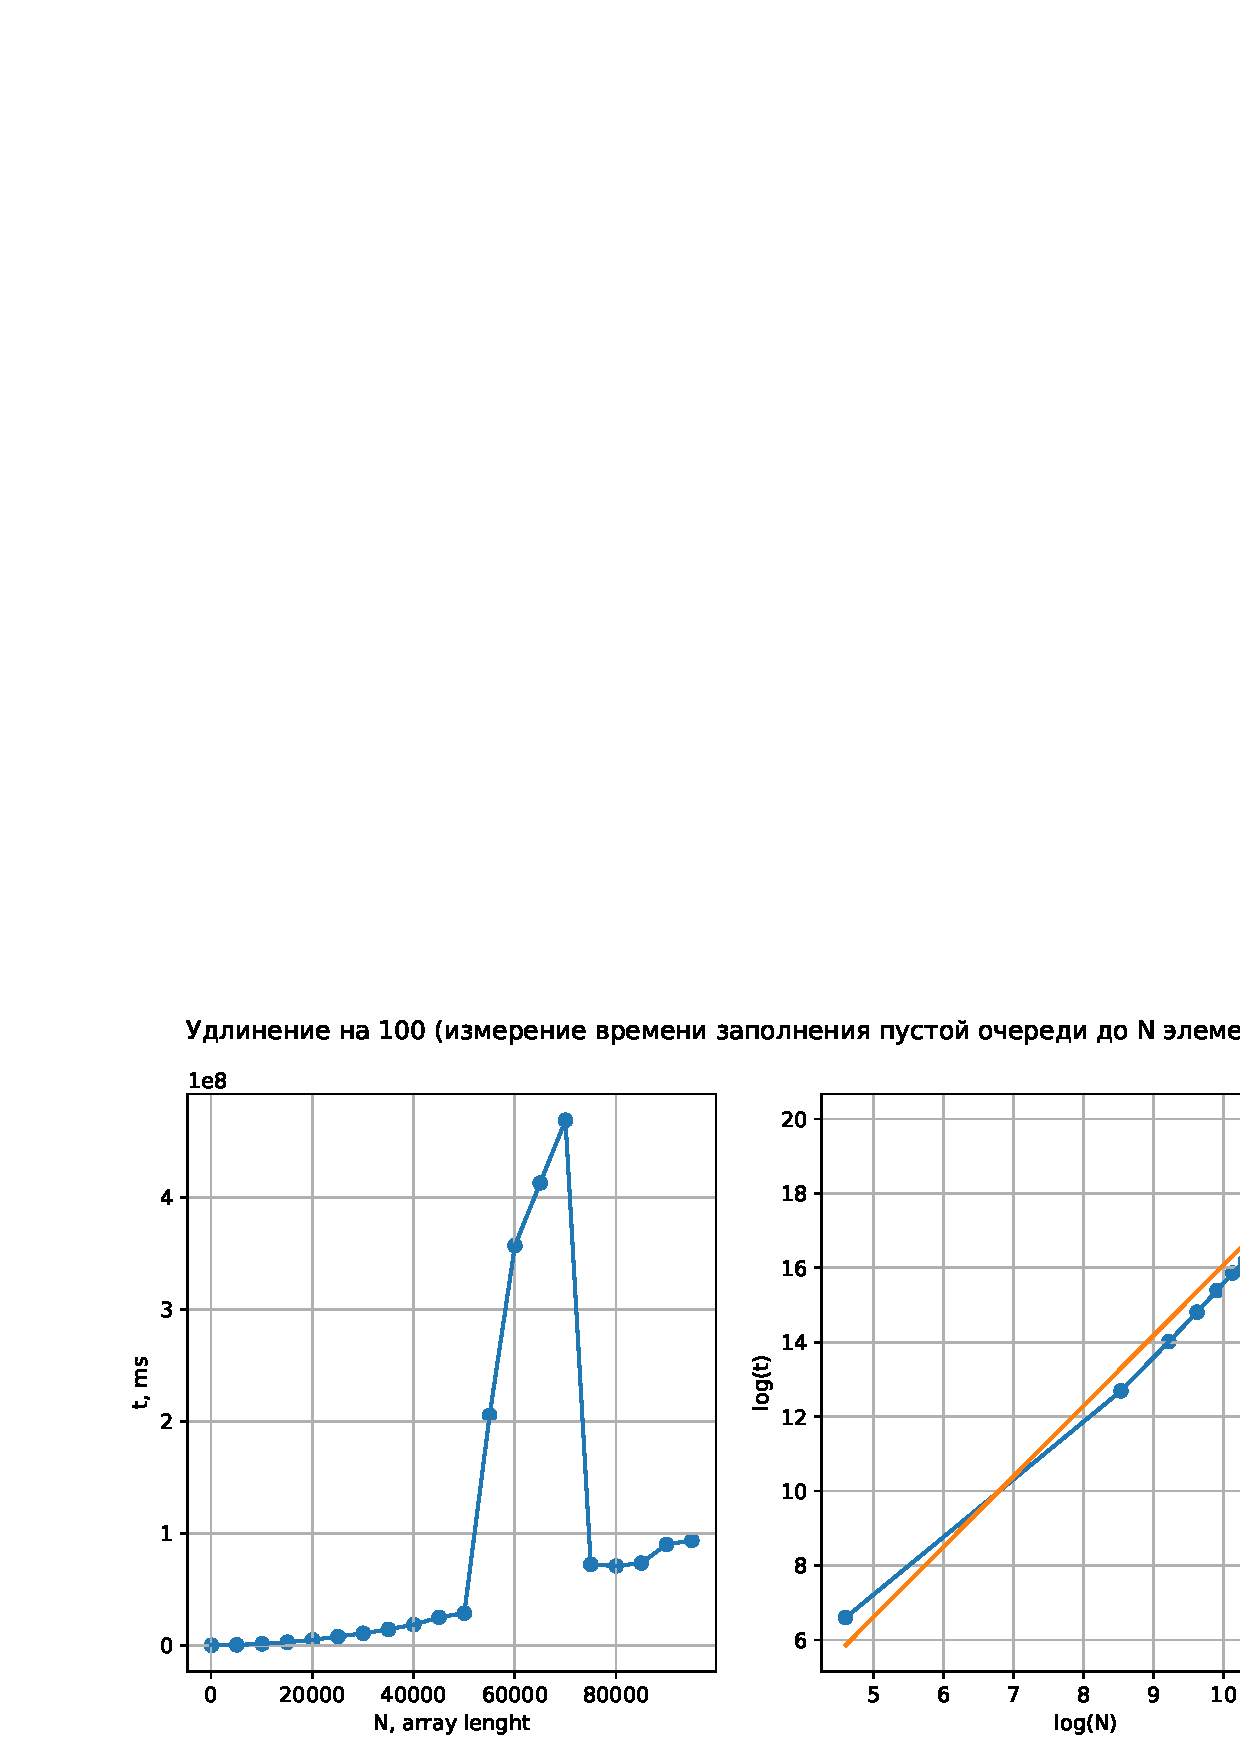
\includegraphics[width=0.9\linewidth]{./bin_search/bin_search.png}}
			\caption{График зависимости времени от длины массива (справа в логарифмическом масштабе)}
			\label{fig:bin_search}
		\end{figure}
	\section*{Сумма двух}
		\par По графику (\figurename\;\ref{fig:sumoftwo}) можно определить, что сложность поиска в отсортированном массиве $O(N)$, а в неотсортированном $O(N^2)$, что совпадает с теоритическими расчетами.
		\begin{figure}[ht!]
			\centering
			{\includegraphics[width=1\linewidth]{./sum_of_two/sumoftwo.png}}
			\caption{График зависимости времени от длины массива (справа в логарифмическом масштабе)}
			\label{fig:sumoftwo}
		\end{figure}
	\section*{Часто используемый элемент}
		
		Как бы грустно это не было, оптимизированные стратегии не дают прироста в скорости ни на равномерном распределении запросов, ни на биномиальном.
		\begin{figure}[ht!]
			\centering
			{\includegraphics[width=1\linewidth]{./freq_used/smart_search.png}}
			\caption{График зависимости времени от длины массива (снизу в логарифмическом масштабе)}
			\label{fig:freq_used}
		\end{figure}
	
	
		\begin{figure}[ht!]
			\centering
			{\includegraphics[width=1\linewidth]{./freq_used/smart_search_with_binomial.png}}
			\caption{График зависимости времени от длины массива (снизу в логарифмическом масштабе)}
			\label{fig:freq_used_binomial}
		\end{figure}
		Действительно, теория говорит тоже самое. Оценим сложность при равномерном распределении запросов:
		$$\dfrac{1+2+\hdots+N}{N} = \dfrac{N(N+1)}{2N} = \dfrac{N+1}{2} = O(N)$$
		А теперь оценим при биномиальном распределении запросов
		$$ \dfrac{1\cdot C^{N}_{2N} + 2C_{2N}^{N-1} + 3C_{2N}^{N+1} + \hdots + NC_{2N}^0}{2N} < \dfrac{2N\cdot C^{N}_{2N} + 2NC_{2N}^{N-1} + 2NC_{2N}^{N+1} + \hdots + 2NC_{2N}^0}{2N} = 2N $$
		С другой стороны по транснеравенству
		$$ \dfrac{1\cdot C^{N}_{2N} + 2C_{2N}^{N-1} + 3C_{2N}^{N+1} + \hdots + NC_{2N}^0}{2N} > \dfrac{1}{2^N}\sum_{n=0}^{2N}nC_{2N}^n = N\dfrac{2^{N-1} - 1}{2^N}$$
		таким образом, это $O(N)$
	\section*{по собственной инициативе}
	Я написал проги, которые делает замер вермени для одного размера массива, и запускал для разных в многопоточке через питон. Получил вот такие красивые графики.(\figurename\;\ref{fig:selfharm})
	
	\begin{figure}[ht!]
		\centering
		\includegraphics[width=0.3\linewidth]{brut999points1workers.jpg}
		\includegraphics[width=0.3\linewidth]{brut999points2workers.jpg}
		\includegraphics[width=0.3\linewidth]{brut999points3workers.jpg}
		\includegraphics[width=0.3\linewidth]{brut999points4workers.jpg}
		\includegraphics[width=0.3\linewidth]{brut999points5workers.jpg}
		\includegraphics[width=0.3\linewidth]{brut999points6workers.jpg}
		\caption{График зависимости времени от длины массива (снизу в логарифмическом масштабе)}
		\label{fig:selfharm}
	\end{figure}
	\section*{Выводы}
		\begin{enumerate}
			\item ассимптотичская сложность может зависеть от входных данных, но не обязательно.
			\item Весь этот бред про "для достаточно больших N" на самом деле работает и для вообразимых величин, но иногда если алгоритм не работает с большими входными данными и в оптимизированном есть много предварительных вычислений, лучше оставить старый.
		\end{enumerate}
\end{document}          
